\begin{figure}
  \centering
  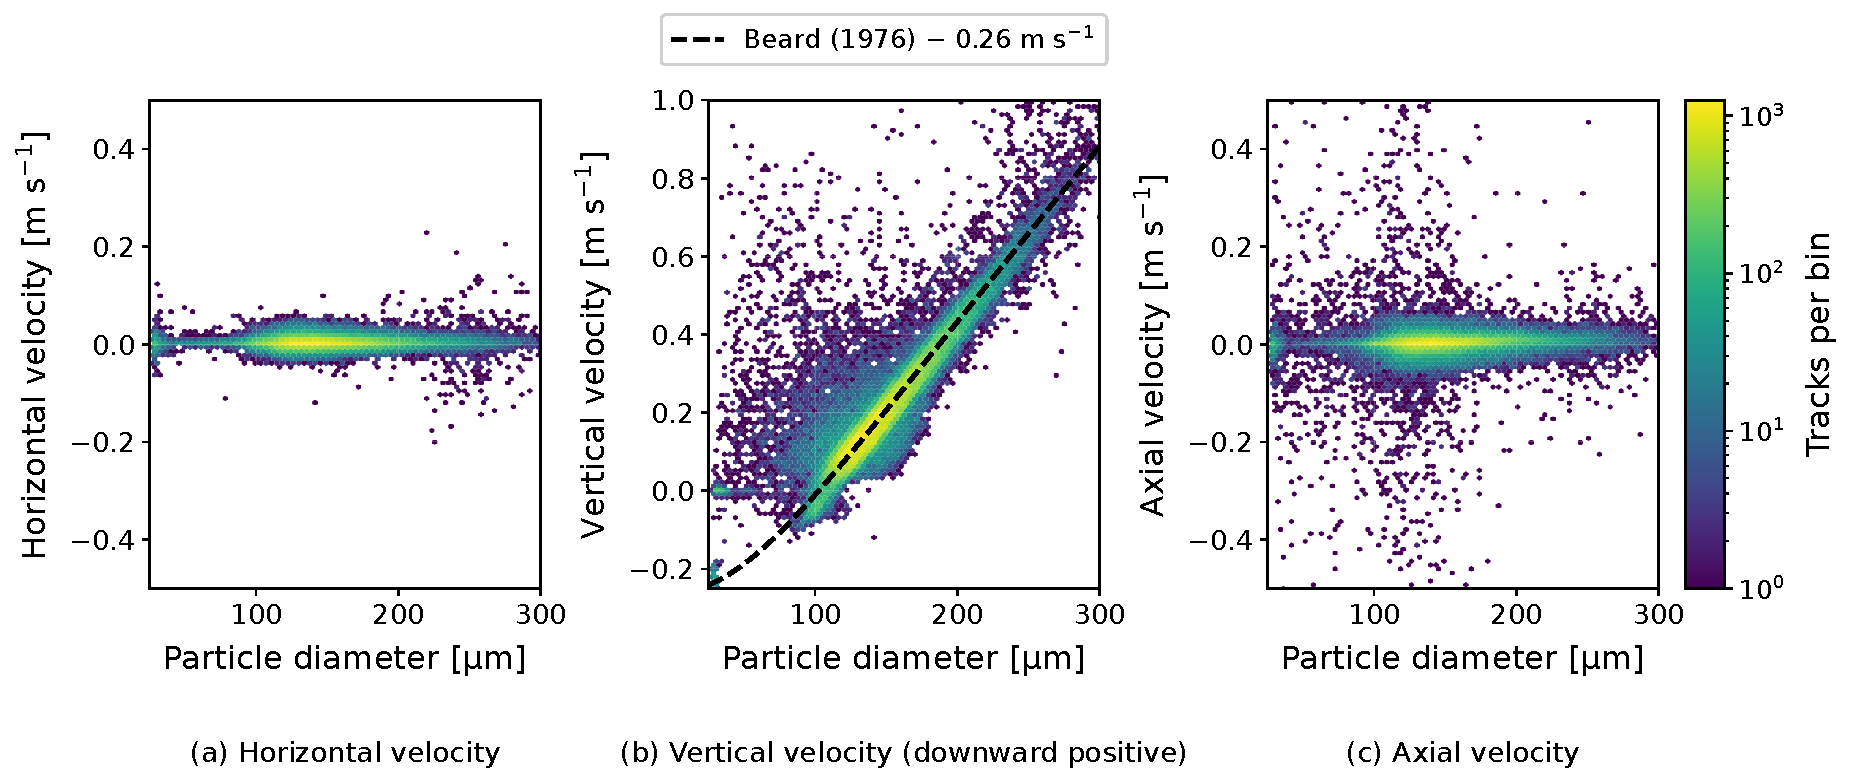
\includegraphics[width=0.98\linewidth]{figures/methods/velocity_distributions_260715.pdf}
  \caption{
    Joint distributions of droplet diameter and velocity obtained from the reconstructed trajectories in the 14 experimental sequences. The panels show the (a) horizontal velocity \(v_x\), (b) vertical velocity \(v_y\), with downward motion defined as positive, and (c) axial velocity \(v_z\), along the optical axis. Color indicates the number of trajectories in each bin on a logarithmic scale. The dashed curve in (b) represents the terminal velocity of Beard (1976), reduced by the mean upward air velocity of \qty{0.26}{\meter\per\second}.
  }
  \label{fig:exp_data_velocity}
\end{figure}
